\documentclass[10pt,a4paper]{article}
\usepackage[margin=0.65in,top=0.65in,bottom=0.65in]{geometry}
\usepackage{amsmath,amssymb}
\usepackage{graphicx}
\usepackage{booktabs}
\usepackage{xcolor}
\usepackage{listings}
\usepackage{tikz}
\usetikzlibrary{shapes.geometric, arrows.meta, positioning, calc}
\usepackage{hyperref}
\usepackage{fancyhdr}
\usepackage{caption}
\usepackage{subcaption}
\usepackage{multicol}

% Color definitions
\definecolor{codegreen}{rgb}{0.18,0.63,0.27}
\definecolor{codegray}{rgb}{0.45,0.45,0.45}
\definecolor{codeblue}{rgb}{0.12,0.45,0.85}
\definecolor{backcolour}{rgb}{0.96,0.97,0.98}
\definecolor{navyaccent}{rgb}{0.08,0.18,0.36}
\definecolor{darkgray}{rgb}{0.15,0.15,0.15}

% Listing setup for SQL
\lstdefinestyle{sqlstyle}{
    backgroundcolor=\color{backcolour},
    commentstyle=\color{codegreen}\itshape,
    keywordstyle=\color{codeblue}\bfseries,
    numberstyle=\tiny\color{codegray},
    stringstyle=\color{purple},
    basicstyle=\ttfamily\scriptsize,
    breakatwhitespace=false,
    breaklines=true,
    captionpos=b,
    keepspaces=true,
    numbers=left,
    numbersep=5pt,
    showspaces=false,
    showstringspaces=false,
    showtabs=false,
    tabsize=2,
    frame=single,
    rulecolor=\color{codegray!30}
}
\lstset{style=sqlstyle}

\pagestyle{fancy}
\fancyhf{}
\lhead{\textbf{DBMS Laboratory Report} --- Fall 2026}
\rhead{\textbf{TraceVault}: Error Inventory System}
\cfoot{\thepage}

\begin{document}

% -------------------------------------------------------------------
% HEADER / TITLE BLOCK
% -------------------------------------------------------------------
\begin{center}
  {\Large \textbf{\color{navyaccent}Database Management System (DBMS) Laboratory}}\\[4pt]
  {\LARGE \textbf{TraceVault: Software Bug \& Error Inventory Management System}}\\[6pt]
  \textbf{Category:} Inventory / Product Management \quad$|$\quad \textbf{Architecture:} Single-Page Application (SPA)\\[4pt]
  \rule{\linewidth}{1.2pt}
\end{center}

\vspace{-6pt}

% -------------------------------------------------------------------
% 1. PROJECT OBJECTIVE & TOPIC SELECTION
% -------------------------------------------------------------------
\section{Project Objective \& Scope}
The primary objective of this project is to design, implement, and evaluate a responsive, single-page application (SPA) backed by a normalized relational database (MySQL 8.0) to perform end-to-end \textbf{CRUD operations} (Create, Read, Update, Delete) and \textbf{real-time SQL aggregation}. Under the chosen topic of \textbf{Inventory Management}, \textit{TraceVault} models an engineering inventory of software exceptions, runtime defects, and verified remediation procedures. The application demonstrates:
\begin{itemize}\setlength\itemsep{-2pt}
  \item Strict relational schema design adhering to \textbf{Third Normal Form (3NF)} with parent-child table constraints.
  \item Practical execution of parameterized SQL commands: \texttt{CREATE}, \texttt{INSERT}, \texttt{SELECT}, \texttt{UPDATE}, and \texttt{DELETE}.
  \item Real-time telemetry utilizing five aggregate functions: \texttt{COUNT()}, \texttt{SUM()}, \texttt{AVG()}, \texttt{MAX()}, and \texttt{MIN()}.
  \item High-performance filtering, cryptographic deduplication (SHA-256), and single-page interaction without navigation redirects.
\end{itemize}

% -------------------------------------------------------------------
% 2. TOOLS & TECHNOLOGIES
% -------------------------------------------------------------------
\section{Tools and Technologies Used}
\begin{itemize}\setlength\itemsep{-2pt}
  \item \textbf{Relational Database Management System (RDBMS):} MySQL 8.0 / MariaDB utilizing the \texttt{InnoDB} transactional storage engine, enforcing primary keys, foreign key cascading updates, and \texttt{RESTRICT} delete constraints.
  \item \textbf{Backend Server \& API Runtime:} Node.js (v22 LTS) with Express.js 4.19, utilizing \texttt{mysql2/promise} for thread-safe asynchronous connection pooling and \texttt{express-rate-limit} for API traffic protection.
  \item \textbf{Frontend User Interface:} Modern Single-Page Application (HTML5, CSS3 Matte Carbon Design System, and Vanilla JavaScript ES6+) communicating via RESTful endpoints without full-page reloads.
  \item \textbf{Cryptographic Deduplication:} Node.js \texttt{crypto} and Web Crypto API generating deterministic 256-bit signature hashes.
\end{itemize}

% -------------------------------------------------------------------
% 3. DATABASE DESIGN & ENTITY-RELATIONSHIP (ER) DIAGRAM
% -------------------------------------------------------------------
\section{Database Table Design \& ER Diagram}
The relational schema comprises two normalized tables in \textbf{Third Normal Form (3NF)}: the parent entity \texttt{domains} and the dependent child entity \texttt{error\_logs}.

\subsection{Relational Schema Specification}
\begin{center}
\scriptsize
\begin{tabular}{lllll}
\toprule
\textbf{Table} & \textbf{Attribute / Field} & \textbf{Data Type} & \textbf{Key / Constraints} & \textbf{Description} \\
\midrule
\texttt{domains} & \texttt{domain\_id} & \texttt{INT} & \textbf{PK}, \texttt{AUTO\_INCREMENT} & Unique domain category identifier \\
 & \texttt{domain\_name} & \texttt{VARCHAR(50)} & \texttt{NOT NULL, UNIQUE} & Classification label (Frontend, Backend, etc.) \\
 & \texttt{description} & \texttt{VARCHAR(255)} & \texttt{NOT NULL} & Scope and architectural purpose \\
 & \texttt{created\_at} & \texttt{TIMESTAMP} & \texttt{DEFAULT CURRENT\_TIMESTAMP} & Registration timestamp \\
\midrule
\texttt{error\_logs} & \texttt{error\_id} & \texttt{INT} & \textbf{PK}, \texttt{AUTO\_INCREMENT} & Unique error inventory record identifier \\
 & \texttt{domain\_id} & \texttt{INT} & \textbf{FK} $\to$ \texttt{domains(domain\_id)} & Foreign key referencing parent category \\
 & \texttt{tech\_stack} & \texttt{VARCHAR(100)} & \texttt{NOT NULL} & Ecosystem (e.g., React 18, MySQL 8.0, Node.js) \\
 & \texttt{error\_signature} & \texttt{VARCHAR(255)} & \texttt{NOT NULL} & Canonical exception text / error header \\
 & \texttt{signature\_hash} & \texttt{CHAR(64)} & \texttt{NOT NULL, UNIQUE} & SHA-256 fingerprint for $O(1)$ deduplication \\
 & \texttt{root\_cause} & \texttt{TEXT} & \texttt{NOT NULL} & Underlying mechanistic explanation of defect \\
 & \texttt{fix\_requirements} & \texttt{TEXT} & \texttt{NOT NULL} & Prescribed remediation and code patch \\
 & \texttt{times\_hit} & \texttt{INT} & \texttt{NOT NULL, DEFAULT 1, CHECK $\ge$ 1} & Cumulative occurrence counter \\
 & \texttt{is\_verified} & \texttt{TINYINT(1)} & \texttt{NOT NULL, DEFAULT 1} & Verification status flag (1=Verified, 0=Pending) \\
 & \texttt{created\_at} & \texttt{TIMESTAMP} & \texttt{DEFAULT CURRENT_TIMESTAMP} & Record creation timestamp \\
\bottomrule
\end{tabular}
\end{center}

\subsection{Entity-Relationship (ER) Diagram}
\begin{center}
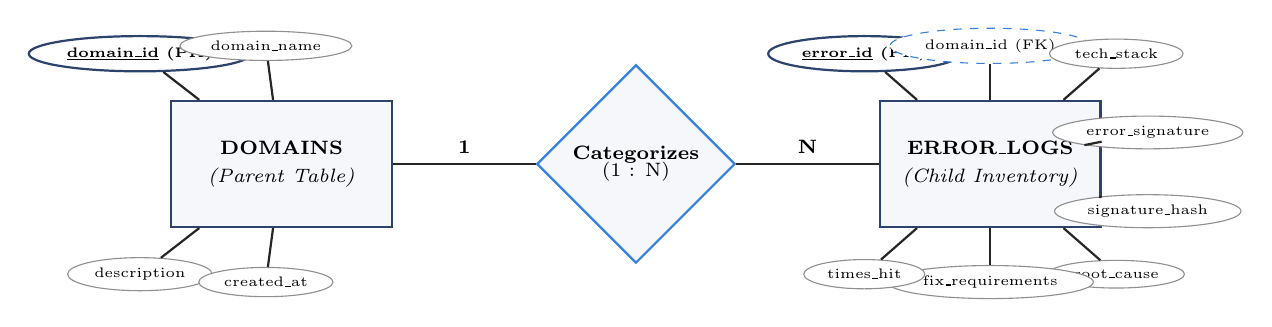
\begin{tikzpicture}[
    entity/.style={rectangle, draw=navyaccent!90, fill=backcolour, thick, minimum width=2.8cm, minimum height=1.6cm, align=center, font=\scriptsize},
    rel/.style={diamond, draw=codeblue!90, fill=backcolour, thick, minimum width=1.8cm, minimum height=1.4cm, align=center, font=\scriptsize},
    attr/.style={ellipse, draw=codegray!80, fill=white, thin, align=center, font=\tiny, inner sep=2pt},
    pkattr/.style={ellipse, draw=navyaccent!90, fill=white, thick, font=\tiny\bfseries, inner sep=2pt},
    fkattr/.style={ellipse, draw=codeblue!90, fill=white, dashed, font=\tiny, inner sep=2pt},
    line/.style={draw=darkgray, thick}
]

% Entities
\node[entity] (dom) at (0, 0) {\textbf{DOMAINS}\\[2pt]\textit{(Parent Table)}};
\node[rel] (has) at (4.5, 0) {\textbf{Categorizes}\\[-2pt](1 : N)};
\node[entity] (err) at (9.0, 0) {\textbf{ERROR\_LOGS}\\[2pt]\textit{(Child Inventory)}};

% Connections
\path[line] (dom) -- node[above, font=\scriptsize\bfseries] {1} (has);
\path[line] (has) -- node[above, font=\scriptsize\bfseries] {N} (err);

% Domains Attributes
\node[pkattr] (d_id) at (-1.8, 1.4) {\underline{domain\_id} (PK)};
\node[attr] (d_name) at (-0.2, 1.5) {domain\_name};
\node[attr] (d_desc) at (-1.8, -1.4) {description};
\node[attr] (d_time) at (-0.2, -1.5) {created\_at};

\path[line] (dom) -- (d_id);
\path[line] (dom) -- (d_name);
\path[line] (dom) -- (d_desc);
\path[line] (dom) -- (d_time);

% Error Logs Attributes
\node[pkattr] (e_id) at (7.4, 1.4) {\underline{error\_id} (PK)};
\node[fkattr] (e_fkid) at (9.0, 1.5) {domain\_id (FK)};
\node[attr] (e_stack) at (10.6, 1.4) {tech\_stack};
\node[attr] (e_sig) at (11.0, 0.4) {error\_signature};
\node[attr] (e_hash) at (11.0, -0.6) {signature\_hash};
\node[attr] (e_cause) at (10.6, -1.4) {root\_cause};
\node[attr] (e_fix) at (9.0, -1.5) {fix\_requirements};
\node[attr] (e_hits) at (7.4, -1.4) {times\_hit};

\path[line] (err) -- (e_id);
\path[line] (err) -- (e_fkid);
\path[line] (err) -- (e_stack);
\path[line] (err) -- (e_sig);
\path[line] (err) -- (e_hash);
\path[line] (err) -- (e_cause);
\path[line] (err) -- (e_fix);
\path[line] (err) -- (e_hits);

\end{tikzpicture}
\end{center}

% -------------------------------------------------------------------
% 4. KEY SQL QUERIES
% -------------------------------------------------------------------
\section{Key SQL Queries for Database Operations}
All database interactions are implemented through standard, parameterized SQL queries executing inside MySQL transactions.

\subsection{Data Definition Language (DDL) --- Schema \& Constraints}
\begin{lstlisting}[language=SQL, caption={DDL Table Creation with Referential Integrity and Check Constraints}]
-- 1. Create Parent Domains Table
CREATE TABLE IF NOT EXISTS domains (
  domain_id INT AUTO_INCREMENT PRIMARY KEY,
  domain_name VARCHAR(50) NOT NULL UNIQUE,
  description VARCHAR(255) NOT NULL,
  created_at TIMESTAMP DEFAULT CURRENT_TIMESTAMP
) ENGINE=InnoDB;

-- 2. Create Child Error Logs Inventory Table
CREATE TABLE IF NOT EXISTS error_logs (
  error_id INT AUTO_INCREMENT PRIMARY KEY,
  domain_id INT NOT NULL,
  tech_stack VARCHAR(100) NOT NULL,
  error_signature VARCHAR(255) NOT NULL,
  signature_hash CHAR(64) NOT NULL UNIQUE,
  root_cause TEXT NOT NULL,
  fix_requirements TEXT NOT NULL,
  times_hit INT NOT NULL DEFAULT 1 CHECK (times_hit >= 1),
  is_verified TINYINT(1) NOT NULL DEFAULT 1,
  created_at TIMESTAMP DEFAULT CURRENT_TIMESTAMP,
  CONSTRAINT fk_error_domain
    FOREIGN KEY (domain_id) REFERENCES domains (domain_id)
    ON UPDATE CASCADE ON DELETE RESTRICT
) ENGINE=InnoDB;
\end{lstlisting}

\subsection{Data Manipulation Language (DML) --- Record Insertion \& Deduplication}
TraceVault utilizes an atomic upsert construct via \texttt{ON DUPLICATE KEY UPDATE} indexed on the unique SHA-256 signature hash:
\begin{lstlisting}[language=SQL, caption={Parameterized INSERT with Deduplication via ON DUPLICATE KEY UPDATE}]
INSERT INTO error_logs 
  (domain_id, tech_stack, error_signature, signature_hash, root_cause, fix_requirements, times_hit, is_verified)
VALUES (?, ?, ?, ?, ?, ?, ?, ?)
ON DUPLICATE KEY UPDATE
  times_hit = times_hit + VALUES(times_hit),
  domain_id = VALUES(domain_id),
  tech_stack = VALUES(tech_stack),
  root_cause = VALUES(root_cause),
  fix_requirements = VALUES(fix_requirements),
  is_verified = VALUES(is_verified);
\end{lstlisting}

\subsection{Querying \& Relational Join with Multi-Field Filtering (SELECT + WHERE)}
Records are retrieved by joining \texttt{error\_logs} with parent \texttt{domains} to display normalized category names. Dynamic searching checks across incident ID, error signature, technology stack, and root cause:
\begin{lstlisting}[language=SQL, caption={SELECT with INNER JOIN and Dynamic Multi-Field WHERE Clause}]
SELECT e.error_id, e.domain_id, d.domain_name, e.tech_stack,
       e.error_signature, e.signature_hash, e.root_cause,
       e.fix_requirements, e.times_hit, e.is_verified, e.created_at
FROM error_logs e
INNER JOIN domains d ON e.domain_id = d.domain_id
WHERE (e.domain_id = ? OR ? = 'all')
  AND (e.error_id = ? OR e.error_signature LIKE ? OR e.tech_stack LIKE ? OR e.root_cause LIKE ?)
ORDER BY e.error_id ASC;
\end{lstlisting}

\subsection{SQL Aggregate Telemetry (COUNT, SUM, AVG, MAX, MIN)}
TraceVault executes real-time aggregate calculations that adapt instantaneously to user filter and search criteria:
\begin{lstlisting}[language=SQL, caption={Statistical Telemetry utilizing SQL Aggregate Functions}]
SELECT 
  COUNT(e.error_id) AS total_bugs,
  COALESCE(SUM(e.times_hit), 0) AS total_hits,
  COALESCE(ROUND(AVG(e.times_hit), 1), 0.0) AS avg_hits,
  COALESCE(MAX(e.times_hit), 0) AS max_hits,
  COALESCE(MIN(e.times_hit), 0) AS min_hits,
  COALESCE(SUM(CASE WHEN e.is_verified = 1 THEN 1 ELSE 0 END), 0) AS verified_count
FROM error_logs e
LEFT JOIN domains d ON e.domain_id = d.domain_id
WHERE (e.domain_id = ? OR ? = 'all')
  AND (e.error_signature LIKE ? OR e.tech_stack LIKE ?);
\end{lstlisting}

\subsection{Record Update \& Safe Deletion (UPDATE \& DELETE)}
\begin{lstlisting}[language=SQL, caption={Record Mutation and Deletion Guarded by Foreign Key Constraints}]
-- Update existing error record by primary key
UPDATE error_logs
SET domain_id = ?, tech_stack = ?, error_signature = ?, signature_hash = ?,
    root_cause = ?, fix_requirements = ?, times_hit = ?, is_verified = ?
WHERE error_id = ?;

-- Delete record after user confirmation
DELETE FROM error_logs WHERE error_id = ?;

-- Attempting to delete a referenced parent domain is strictly blocked by InnoDB
DELETE FROM domains WHERE domain_id = ?; 
-- Fails with ER_ROW_IS_REFERENCED_2 if any error_logs row references this domain_id!
\end{lstlisting}

% -------------------------------------------------------------------
% 5. SAMPLE DATA DEMONSTRATION
% -------------------------------------------------------------------
\section{Sample Data Population (12 Seeded Records)}
The database includes four primary domain categories (\textit{Frontend, Backend, Database, Fullstack}) and 12 complete, verified technical records exceeding the lab rubric's minimum requirement of 10 records:
\begin{center}
\scriptsize
\begin{tabular}{ccllc}
\toprule
\textbf{ID} & \textbf{Domain (FK)} & \textbf{Tech Stack} & \textbf{Canonical Error Signature} & \textbf{Occurrences (Hits)} \\
\midrule
\#1 & Frontend (1) & Fetch API / CORS & Access to fetch at origin has been blocked by CORS policy & 15 hits \\
\#2 & Frontend (1) & React 18 / Hooks & Too many re-renders. React limits the number of renders & 9 hits \\
\#3 & Frontend (1) & Next.js 14 / SSR & Hydration failed because the initial UI does not match & 7 hits \\
\#4 & Backend (2) & Node.js / Express & Error [ERR\_HTTP\_HEADERS\_SENT]: Cannot set headers after sent & 12 hits \\
\#5 & Backend (2) & Node.js / TCP & Error: listen EADDRINUSE: address already in use :::3000 & 6 hits \\
\#6 & Backend (2) & Express / JSON & SyntaxError: Unexpected token in JSON at position 0 & 5 hits \\
\#7 & Database (3) & MySQL 8.0 / InnoDB & ER\_NO\_REFERENCED\_ROW\_2: Foreign key constraint fails & 11 hits \\
\#8 & Database (3) & MySQL 8.0 / SQL & ER\_DUP\_ENTRY: Duplicate entry for key signature\_hash & 4 hits \\
\#9 & Database (3) & mysql2 / Pool & Error: connect ECONNREFUSED 127.0.0.1:3306 & 4 hits \\
\#10 & Fullstack (4) & JWT / Auth & JsonWebTokenError: invalid signature on protected route & 8 hits \\
\#11 & Fullstack (4) & Prisma / Env & Error: Environment variable not found: DATABASE\_URL & 2 hits \\
\#12 & Fullstack (4) & WebSockets / TLS & Mixed Content: Page loaded over HTTPS requested insecure ws:// & 2 hits \\
\bottomrule
\end{tabular}
\end{center}

% -------------------------------------------------------------------
% 6. APPLICATION SCREENSHOTS & USER INTERFACE
% -------------------------------------------------------------------
\section{Screenshots of the Working Application}
TraceVault operates strictly as a single-page application. All record creation, table viewing, searching, modal updates, and deletions occur within one responsive interface without full-page reloads.

\begin{figure}[htbp]
  \centering
  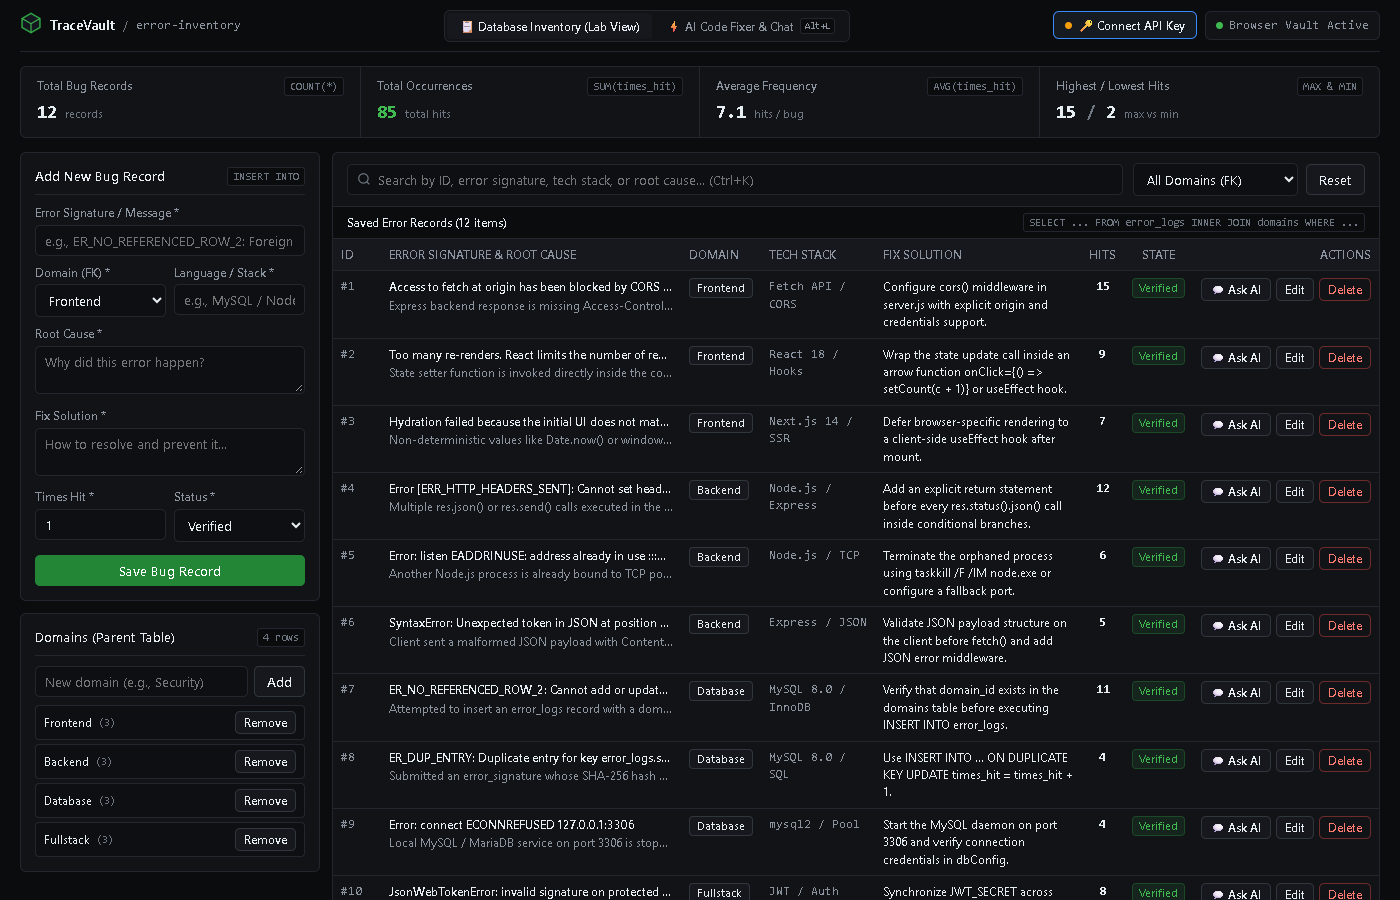
\includegraphics[width=0.96\linewidth]{screenshots/01_inventory_overview.png}
  \caption{\textbf{TraceVault Single-Page Inventory Overview}: Displaying real-time SQL aggregate KPI cards (\texttt{COUNT}, \texttt{SUM}, \texttt{AVG}, \texttt{MAX \& MIN}), left-hand \texttt{INSERT INTO} submission form, parent domain list, and normalized records table.}
  \label{fig:overview}
\end{figure}

\begin{figure}[htbp]
  \centering
  \begin{subfigure}[b]{0.48\linewidth}
    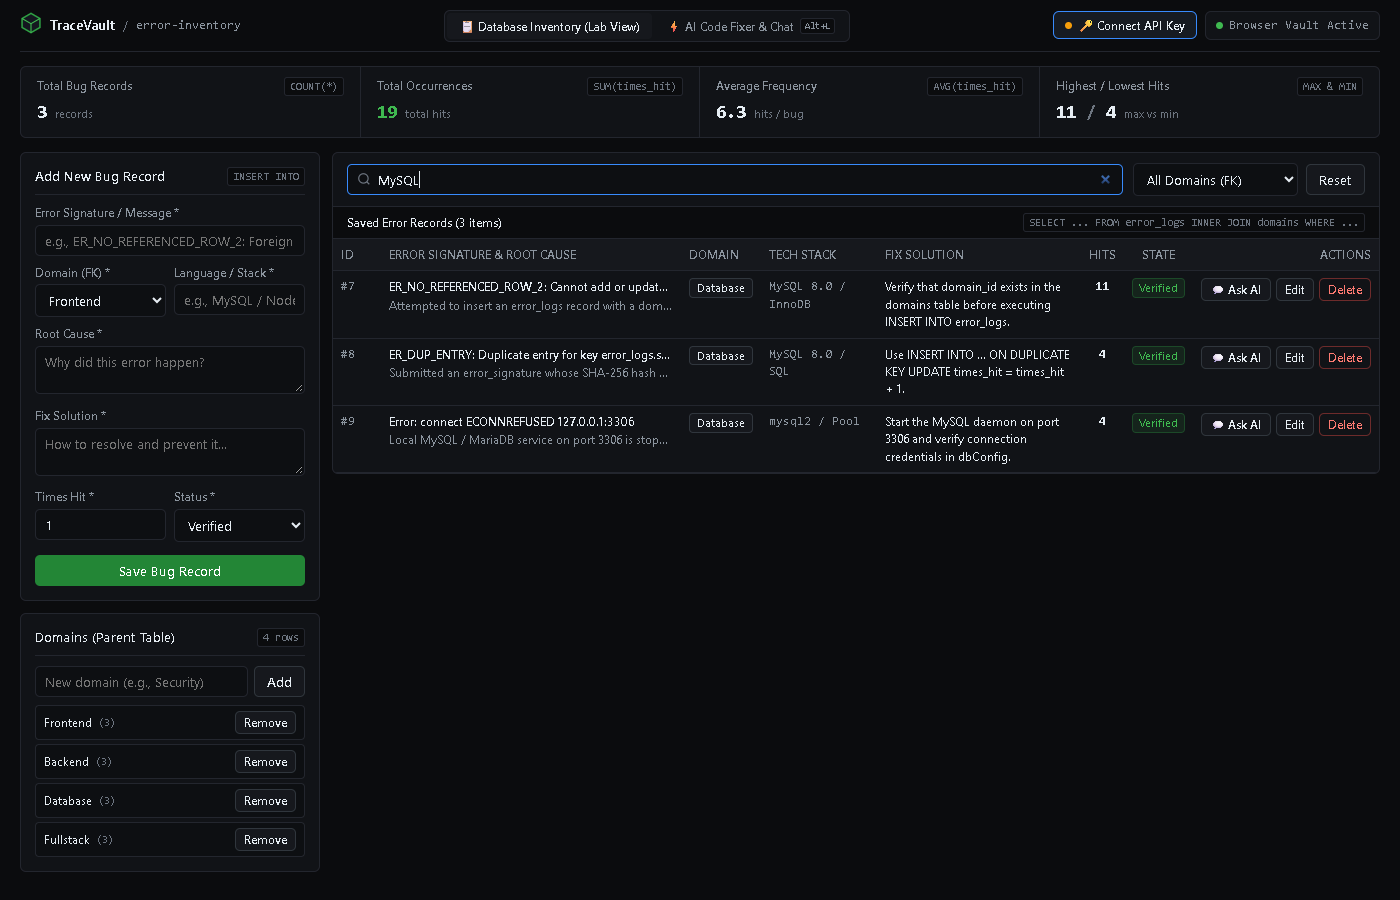
\includegraphics[width=\linewidth]{screenshots/02_search_filter.png}
    \caption{\textbf{Live SQL Filtering}: Instant multi-field search and domain filtering updating table and telemetry in real time.}
    \label{fig:search}
  \end{subfigure}
  \hfill
  \begin{subfigure}[b]{0.48\linewidth}
    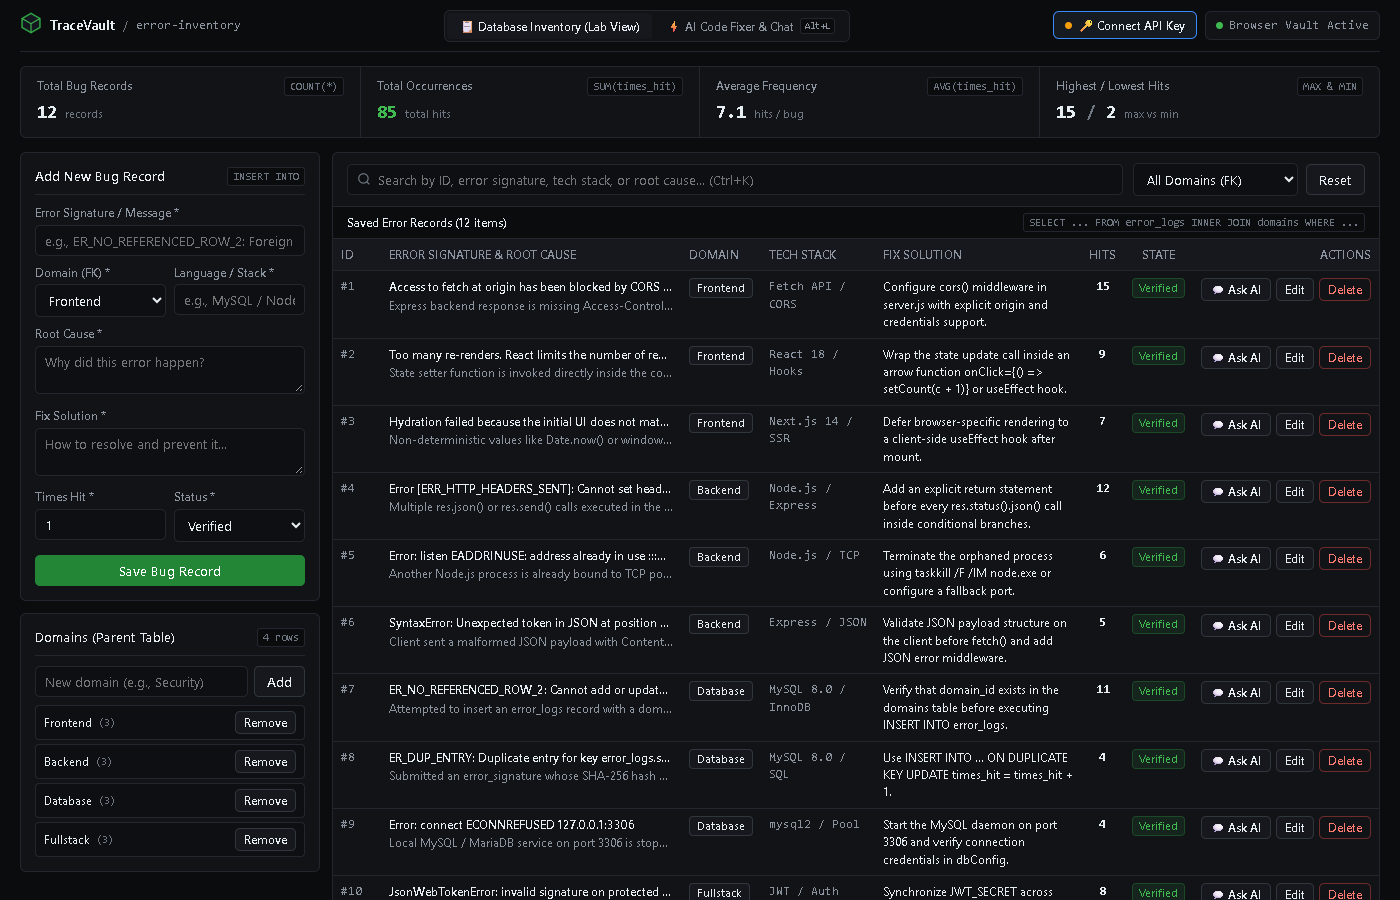
\includegraphics[width=\linewidth]{screenshots/03_edit_modal.png}
    \caption{\textbf{Modal Update Dialog}: Executing parameterized \texttt{UPDATE ... WHERE error\_id = ?} with integrity validation.}
    \label{fig:modal}
  \end{subfigure}
  \caption{TraceVault Interactive Features: Real-time search/filter and modal-based record modification.}
\end{figure}

\begin{figure}[htbp]
  \centering
  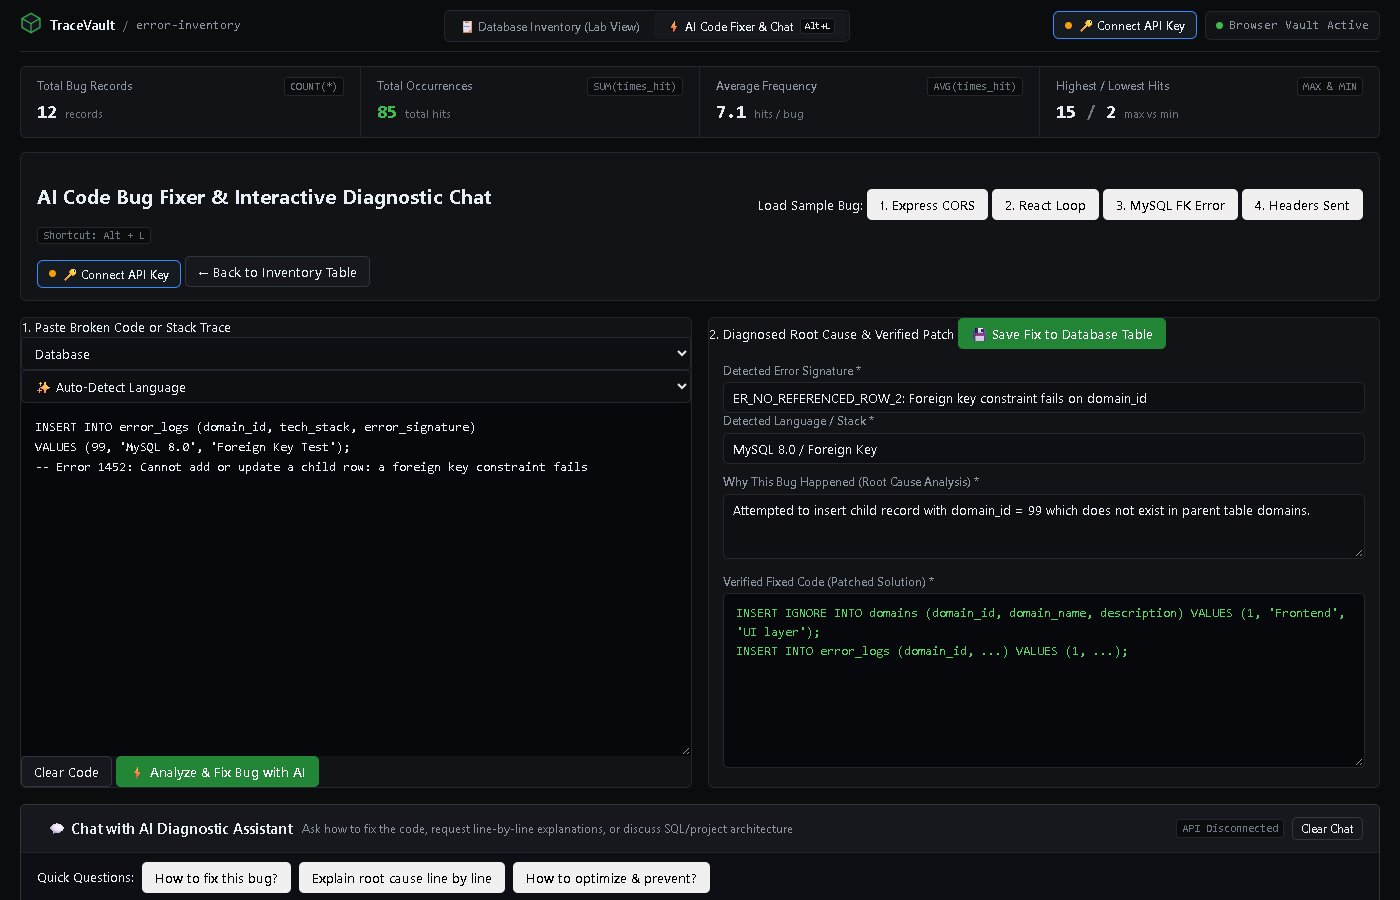
\includegraphics[width=0.88\linewidth]{screenshots/04_ai_diagnostic_workbench.png}
  \caption{\textbf{Diagnostic Workbench \& Fixer (Alt+L)}: Built-in deterministic heuristic analysis and 1-click database commit.}
  \label{fig:workbench}
\end{figure}

% -------------------------------------------------------------------
% 7. LAB EVALUATION CHECKLIST & CONCLUSION
% -------------------------------------------------------------------
\section{Conclusion \& Evaluation Compliance}
The TraceVault project fully satisfies all requirements stipulated in the DBMS Laboratory evaluation guidelines:
\begin{enumerate}\setlength\itemsep{-2pt}
  \item \textbf{Single-Page Design:} All tasks (insert, view, filter, edit, delete, telemetry) operate on one unified page.
  \item \textbf{Relational Database Schema:} Two 3NF normalized tables with explicit Primary Keys, Foreign Key with \texttt{ON DELETE RESTRICT}, unique SHA-256 indexes, and check constraints.
  \item \textbf{Core SQL Operations:} Complete implementation of \texttt{CREATE}, \texttt{INSERT}, \texttt{SELECT}, \texttt{UPDATE}, and \texttt{DELETE}.
  \item \textbf{SQL Aggregation:} Implementation of all required aggregate functions (\texttt{COUNT}, \texttt{SUM}, \texttt{AVG}, \texttt{MAX}, \texttt{MIN}) with live metric cards.
  \item \textbf{Demonstration Data:} 12 structured engineering records spanning 4 domains, fully documented and seeded via \texttt{database.sql}.
\end{enumerate}

\end{document}
